\documentclass[border=10pt]{standalone}
\usepackage[svgnames]{xcolor}
\usepackage{amsmath}
\usepackage{pgfplots}
\pgfplotsset{compat=newest}
\usepackage[sfdefault]{FiraSans}
\usepackage{FiraMono}
\renewcommand*\familydefault{\sfdefault}
\begin{document}
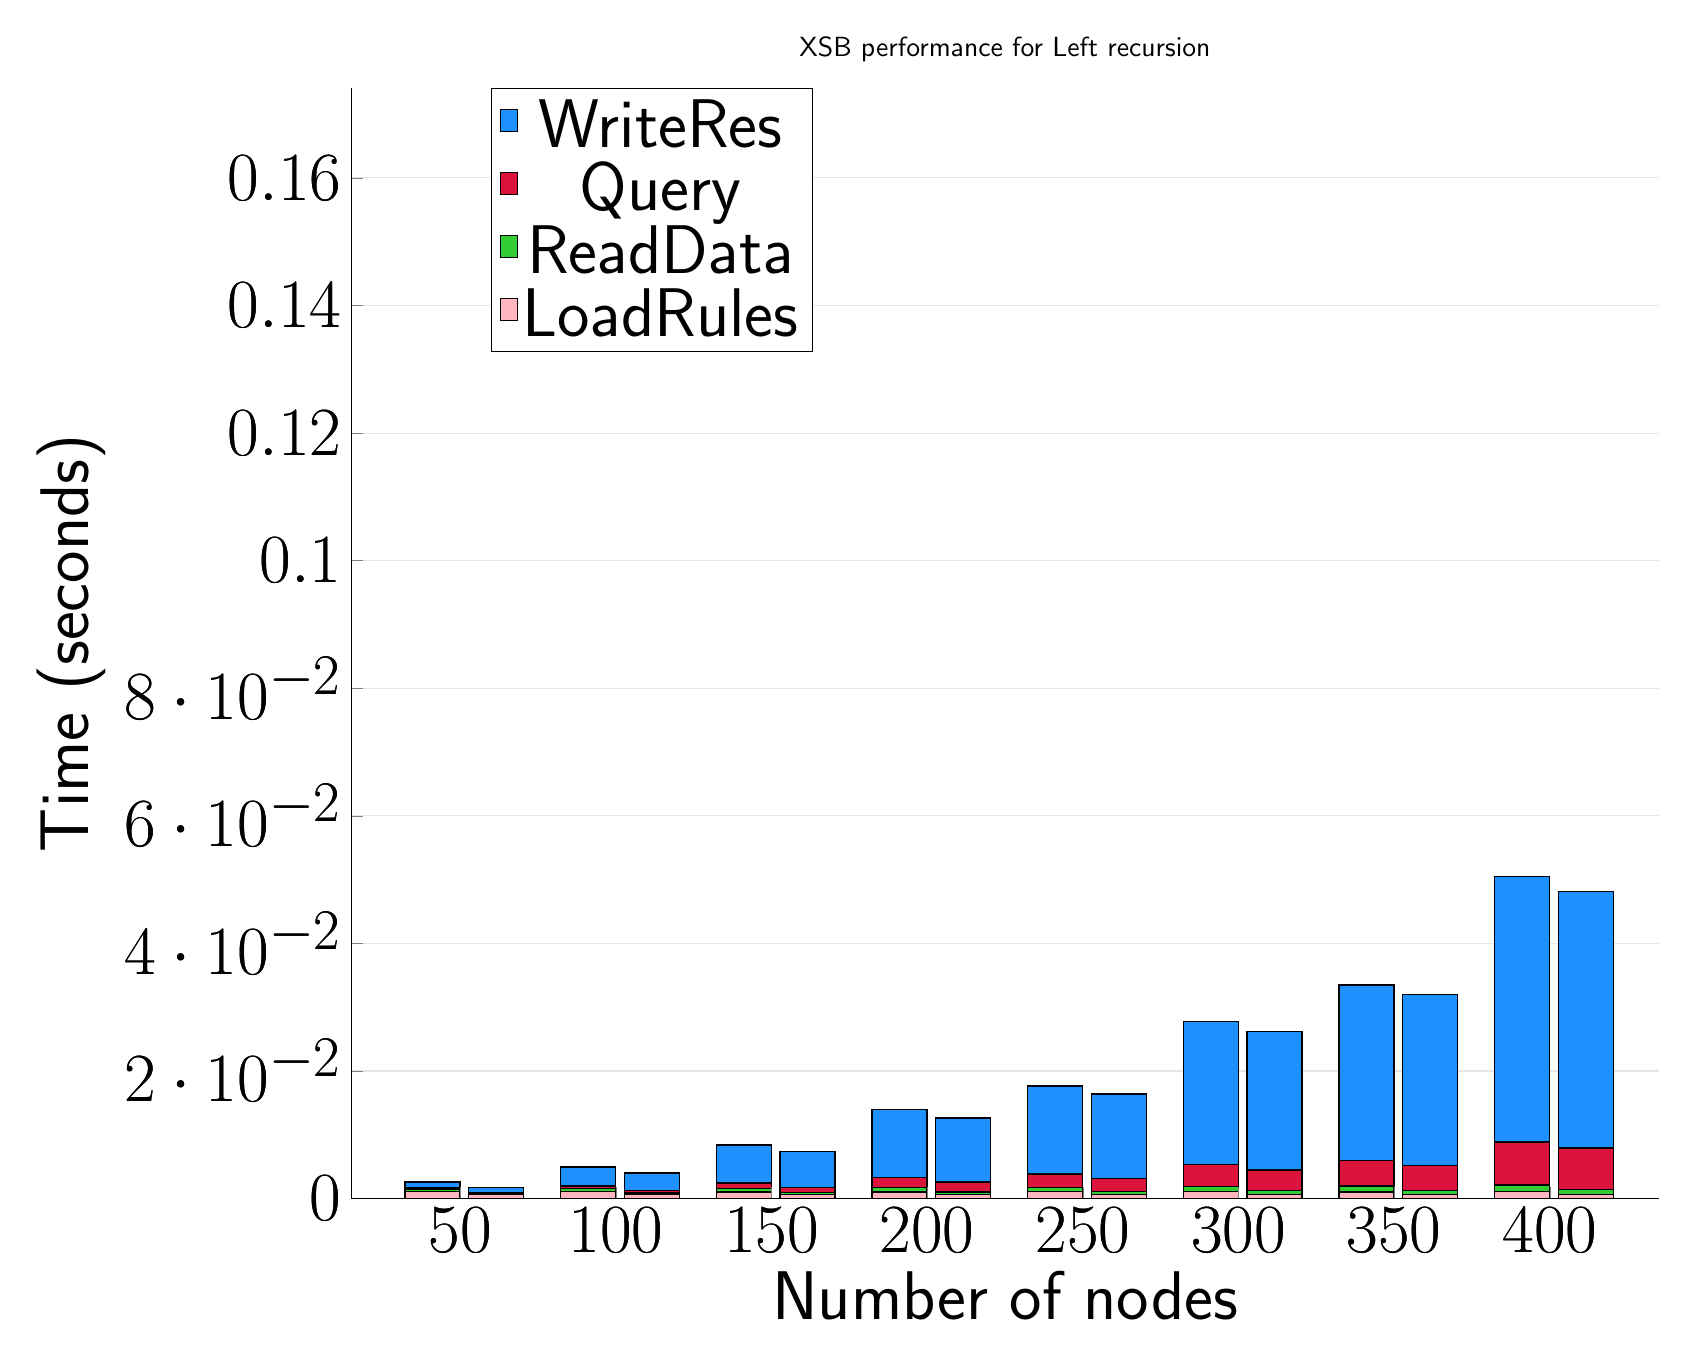
\begin{tikzpicture}
\begin{axis}[
   ybar stacked,
   title={XSB performance for Left recursion},
   bar shift=-10pt,
   width=1.5\textwidth,
   bar width=0.7cm,
   ymajorgrids, tick align=inside,
   major grid style={draw=gray!20},
   xtick=data,
   ymin=0, ymax=0.1741104793548585,
   axis x line*=bottom,
   axis y line*=left,
   enlarge x limits=0.1,
   legend style={
       at={(0.23, 1)},
       anchor=north,
       legend columns=1,
       font=\Huge,
   },
   ylabel={Time (seconds)},
   xlabel={Number of nodes},
   label style={font=\Huge},
   tick label style={font=\Huge},
]
\addlegendimage{fill=DodgerBlue, draw=black, line width=0.2pt}
\addlegendentry{WriteRes}
\addlegendimage{fill=Crimson, draw=black, line width=0.2pt}
\addlegendentry{Query}
\addlegendimage{fill=LimeGreen, draw=black, line width=0.2pt}
\addlegendentry{ReadData}
\addlegendimage{fill=LightPink, draw=black, line width=0.2pt}
\addlegendentry{LoadRules}
\addplot +[fill=LightPink, draw=black, line width=0.5pt] coordinates {
    (50, 0.001088309288024903)
    (100, 0.0010833024978637701)
    (150, 0.00103304386138916)
    (200, 0.001044416427612304)
    (250, 0.001060891151428223)
    (300, 0.001069664955139163)
    (350, 0.001043295860290527)
    (400, 0.0010663986206054681)
};
\addplot +[fill=LimeGreen, draw=black, line width=0.5pt] coordinates {
    (50, 0.0004317998886108398)
    (100, 0.0004849910736083983)
    (150, 0.000568509101867676)
    (200, 0.0006494998931884765)
    (250, 0.0007127046585083007)
    (300, 0.0008465290069580078)
    (350, 0.0009044170379638672)
    (400, 0.001041412353515625)
};
\addplot +[fill=Crimson, draw=black, line width=0.5pt] coordinates {
    (50, 0.0001205921173095701)
    (100, 0.00042798519134521493)
    (150, 0.0008541107177734375)
    (200, 0.001588201522827147)
    (250, 0.002084207534790038)
    (300, 0.0033926725387573254)
    (350, 0.004037714004516603)
    (400, 0.006747531890869139)
};
\addplot +[fill=DodgerBlue, draw=black, line width=0.5pt] coordinates {
    (50, 0.0009670257568359378)
    (100, 0.0029478549957275392)
    (150, 0.005940628051757814)
    (200, 0.01065702438354491)
    (250, 0.013782072067260741)
    (300, 0.02245953083038329)
    (350, 0.027497506141662603)
    (400, 0.04161412715911866)
};
\end{axis}
\begin{axis}[
   ybar stacked,
   bar shift=13pt,
   width=1.5\textwidth,
   bar width=0.7cm,
   ymajorgrids, tick align=inside,
   major grid style={draw=none},
   xtick=data,
   ymin=0, ymax=0.1741104793548585,
   axis x line*=none,
   axis y line*=none,
   enlarge x limits=0.1,
   label style={font=\Huge},
   tick label style={font=\Huge},
]
\addplot +[fill=LightPink, draw=black, line width=0.5pt] coordinates {
    (50, 0.0006234)
    (100, 0.0006140000000000003)
    (150, 0.0005979000000000003)
    (200, 0.0006039000000000003)
    (250, 0.0006099000000000002)
    (300, 0.0006162999999999999)
    (350, 0.0006065000000000005)
    (400, 0.0006103999999999998)
};
\addplot +[fill=LimeGreen, draw=black, line width=0.5pt] coordinates {
    (50, 0.0002159999999999999)
    (100, 0.00028549999999999973)
    (150, 0.00035489999999999995)
    (200, 0.0004419999999999997)
    (250, 0.0004924999999999992)
    (300, 0.0006106999999999998)
    (350, 0.0006636000000000005)
    (400, 0.0007914000000000008)
};
\addplot +[fill=Crimson, draw=black, line width=0.5pt] coordinates {
    (50, 0.00011319999999999969)
    (100, 0.0004071)
    (150, 0.0008225000000000003)
    (200, 0.0015279)
    (250, 0.002016)
    (300, 0.0032730000000000003)
    (350, 0.0039008000000000003)
    (400, 0.0065328999999999995)
};
\addplot +[fill=DodgerBlue, draw=black, line width=0.5pt] coordinates {
    (50, 0.0007389999999999999)
    (100, 0.0026892)
    (150, 0.0055813)
    (200, 0.0100794)
    (250, 0.013255799999999998)
    (300, 0.021685199999999998)
    (350, 0.0267913)
    (400, 0.0402019)
};
\end{axis}
\end{tikzpicture}

\end{document}
